\documentclass{beamer}
\usepackage[orientation=portrait,size=a0,scale=1.4,debug]{beamerposter}
\mode<presentation>{\usetheme{RWTH2}}
\usepackage{chemformula}
\usepackage[utf8]{inputenc}
\usepackage[german, english]{babel} % required for rendering German special characters
\usepackage{siunitx} %pretty measurement unit rendering
\usepackage{hyperref} %enable hyperlink for urls
\usepackage{ragged2e}
\usepackage[font=scriptsize,justification=justified]{caption}
\usepackage{array,booktabs,tabularx}
\usepackage[autostyle=true,german=quotes,english=american]{csquotes}

\usepackage{amsmath, mhchem} % Unterstützung für mathematische und chemische Formeln

\usepackage{floatflt}

\usepackage[authoryear]{natbib}
\bibliographystyle{apalike}

\newcolumntype{Z}{>{\centering\arraybackslash}X} % centered tabularx columns
\sisetup{per=frac,fraction=sfrac}

\title{\ Summer School \enquote{CCS~in~the~High~North}}
%\author{Marco van Veen$^{1}$}
%\institute[RWTH Aachen University]{$^{1}$Institute of Computational Geoscience and Reservoir Engineering, RWTH Aachen University, Germany}
\author{Marco van Veen$^{1}$, Andrew Steadman$^{2}$, Valentin Zuchuat$^{3}$}
\institute[RWTH Aachen University]{$^{1}$Institute of Computational Geoscience and Reservoir Engineering, RWTH Aachen University, Germany\\
$^{2}$School of Earth Sciences, University of Bristol, United Kingdom\\
$^{3}$Department of Geosciences, University of Oslo, Norway
}
\date{\today}

% edit this depending on how tall your header is. We should make this scaling automatic :-/
\newlength{\columnheight}
\setlength{\columnheight}{104cm}

\begin{document}
\begin{frame}

\begin{columns}

	\begin{column}{.382\textwidth}
		\begin{beamercolorbox}[center]{postercolumn}
			\begin{minipage}{.98\textwidth}  % tweaks the width, makes a new \textwidth
				\parbox[t][\columnheight]{\textwidth}{ % must be some better way to set the the height, width and textwidth simultaneously
				
				
				
				
				
				
				
				
\begin{myblock}{Introduction}

\textbf{Carbon Capture and Storage (CCS) is one of the major mitigation measures to handle climate change. Even though international organisations agreed on the importance of CCS and the effective Paris Agreement refers to the widely accepted climate scenarios, the technology is not implemented on a large scale beyond pilot projects yet, nor are economic incentives given to foster its deployment. CCS is not a cutting-edge technology, the applied methods are well-known – not only in the oil and gas industry. Buzz words like enhanced oil recovery (EOR) and carbon capture, utilisation and storage (CCUS) stir up hope to realise large-scale projects soon and in an economically viable way.}
						\vspace{0.5em}
						\begin{figure}
							\begin{minipage}{0.95\textwidth}
								\centering\includegraphics[width=1\textwidth]{figures/photos/group.jpg}
								\caption{Students of 2016 at the edge of the world's northernmost swimming pool in the abandoned Russian mining town of Pyramiden (Photo: V. Zuchuat).}
								\label{fig:group}
							\end{minipage}
						\end{figure}


The summer school \enquote{CCS in the High North} is a collaboration between the \textbf{University of Oslo} (UiO), the \textbf{Colorado School of Mines} (CSM) in Golden and the \textbf{University Centre in Svalbard} (UNIS). It offers a suite of lectures, exercises and geological field work on MSc and PhD level, which are credited with \textbf{13 ECTS}. A highly motivated group of international students with diverse backgrounds and specialisations were not only taught, but also engaged themselves in inspiring discussions.

%Unfortunately, in 2017 the course in Golden, Colorado had to be cancelled due to high political uncertainties and visa restrictions for international students.
\end{myblock}\vfill
					
					
					
					
\begin{myblock}{Course Content}

	
\includegraphics[scale=0.1]{figures/icons/eco_law}~\textbf{Economy, Policies \& Risk}
	\begin{itemize}
		\item The need for CCS: Physics, history and challenges of global climate change
		\item Economics and regulations: Incentives, carbon trading, \ce{CO2} utilisation
		\item Risk Assessment: Monitoring, simulation and liability
	\end{itemize}
	\vspace{0.5em}
						
	

	
\includegraphics[scale=0.1]{figures/icons/geo}~\textbf{Geology \& Reservoir}
	\begin{itemize}
		\item Trapping mechanisms \& storage options: Static vs. dynamic storage
		\item Geological reservoir characterisation: Field observations and core logging
		\item Seal properties: Mechanical and chemical compaction, global data collections and experimental studies
		\item Rock mechanics: Fractures, secondary permeability
		\item Risk of fault and fracture leakage: Sub-seismic resolution, juxtaposition, smearing
	\end{itemize}
	\vspace{0.5em}
	
	
\includegraphics[scale=0.1]{figures/icons/tech}~\textbf{Technology}
	\begin{itemize}
		\item Physical and chemical properties of \ce{CO2}
		\item Separation technologies: Chemical absorption, phase change, polymeric membranes
		\item Enhanced Oil Recovery: Relative permeability \& mobility ratio
		\item Sequestration modelling: Rock \& fluid properties, multi-phase flow, initialisation, events/wells
	\end{itemize}
	
						
\end{myblock}
					
					
		}\end{minipage}\end{beamercolorbox}
	\end{column}



	\begin{column}{.618\textwidth}
		\begin{beamercolorbox}[center]{postercolumn}
			\begin{minipage}{.98\textwidth} % tweaks the width, makes a new \textwidth
				\parbox[t][\columnheight]{\textwidth}{ % must be some better way to set the the height, width and textwidth simultaneously








					
					
					
					
					
\begin{myblock}{Fieldwork \& The Longyearbyen \ce{CO2} Lab}
Highlight of the Summer School were three days of fieldwork on the Arctic archipelago of Svalbard. The aim of the field investigations was to identify potential reservoir formations, evaluate and compare them on their ability to safely store \ce{CO2}. Beside two promising \ce{CO2} storage formations (see figures \ref{fig:fieldwork_adolfbukta} and \ref{fig:fieldwork_skansbukta}), also the targeted units of the Longyearbyen \ce{CO2} Lab were logged in the field close to Deltanesset. Tight sandstones with quartz-overgrowth and pore-filling clay minerals can be observed. Mudstone layers, a thrust décollement and lateral permafrost provide sufficient sealing (compare figure \ref{fig:cross_section}). Injection tests show secondary permeability caused by fractures and the sealing ability is proven by high underpressure in the reservoir \citep{braathen_longyearbyen_2012}.
	\vspace{0.5em}
	\begin{figure}
		\begin{minipage}{0.95\textwidth}
			\begin{minipage}[t]{0.32\textwidth}
				\centering\includegraphics[width=1\textwidth]{figures/photos/arrival_adolfbukta}
				\caption{Going ashore in Adolfbukta: Survival suits, rifles, redundant communications and an emergency backpack are essential HSE equipment during fieldwork on the Arctic archipelago of Svalbard (Photo: M.\,Gutierrez).}
				\label{fig:arrival_adolfbukta}
			\end{minipage}
			\hspace{\fill}
			\begin{minipage}[t]{0.32\textwidth}
				\centering\includegraphics[width=1\textwidth]{figures/photos/fieldwork_adolfbukta}
				\caption{Exposed sandstones of the Carboniferous Ebbadalen Formation north of Adolfbukta. Seven distinctive coarsening-up sequences of thick beds alternating with silty layers are expected to provide high horizontal permeability (Photo: M.\,Gutierrez).}
				\label{fig:fieldwork_adolfbukta}
			\end{minipage}
			\hspace{\fill}
			\begin{minipage}[t]{0.32\textwidth}
				\centering\includegraphics[width=1\textwidth]{figures/photos/fieldwork_skansbukta}
				\caption{Permian limestone beds of the Gipshuken and Kapp Starostin Formations are found at Skansbukta. Bioturbation structures filled with evaporitic material could provide secondary porosity. The picture shows cross-bedding in upper layers (Photo: M.\,Gutierrez).}
				\label{fig:fieldwork_skansbukta}
			\end{minipage}	
		\end{minipage}
	\end{figure}
	\vspace{0.2em}



	\begin{figure}
		\begin{minipage}{.94\textwidth}
			\centering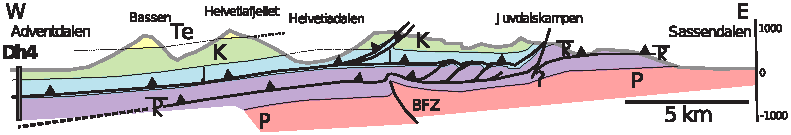
\includegraphics[width=\textwidth]{figures/cross_section}
			\caption{Cross section of the targeted storage formation (Upper Triassic–Middle Jurassic sandstones of the Kapp Toscana Group), the overlying seal (Jurassic mudstones of the Agardfjellet Formation) and the prominent thrust décollement which is providing an additional seal. The indicated well Dh4 in the west is part of the Longyearbyen \ce{CO2} Lab, the logging took place in the east where the layers are outcropping. Modified from \cite{braathen_longyearbyen_2012}.}
			\label{fig:cross_section}
		\end{minipage}
	\end{figure}
%	\vspace{0.4em}

\end{myblock}\vfill					
				
				
\begin{myblock}{Limited Information \& Seal Uncertainty}

\vspace{0.3em}
\begin{figure}
	\begin{minipage}{0.95\textwidth}
		\begin{minipage}[t]{0.36\textwidth}
			\vspace{0pt}
			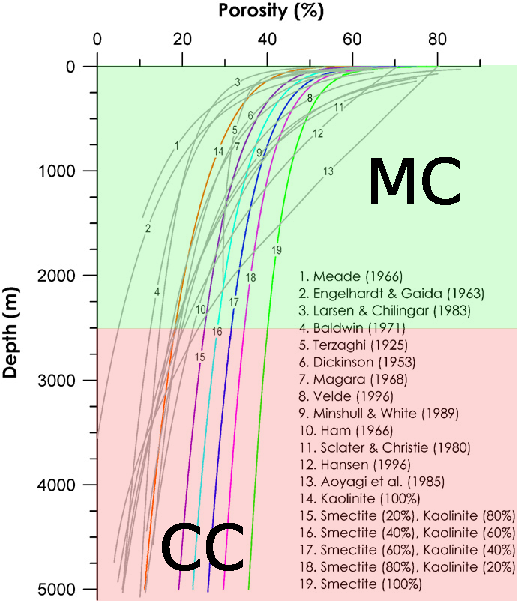
\includegraphics[width=\textwidth]{figures/compaction.pdf}
		\end{minipage}\hfill
		\begin{minipage}[t]{0.22\textwidth}
			\vspace{0pt}
			\caption{
			Comparison of porosity–depth trend studies and experimental results for shales and
argillaceous sediments. While for E\&P projects the seal integrity is proven by the abundance of hydrocarbons, for \ce{CO2} storage it remains uncertain. Controlling factors are clay mineral and pore fluid composition, grain sizes, pore pressure and the influence of mechanical \textbf{(MC)} and chemical compaction \textbf{(CC)}. Because core sampling of seal layers is expensive, experimental studies and global databases might be auxiliary. Still, extrapolation of experimental results has limited validity for natural anisotropy and the influence of chemical compaction \citep{mondol_experimental_2007}.
			} \label{fig:compaction}
		\end{minipage}\hfill
		\begin{minipage}[t]{0.38\textwidth}
			\vspace{0pt}
			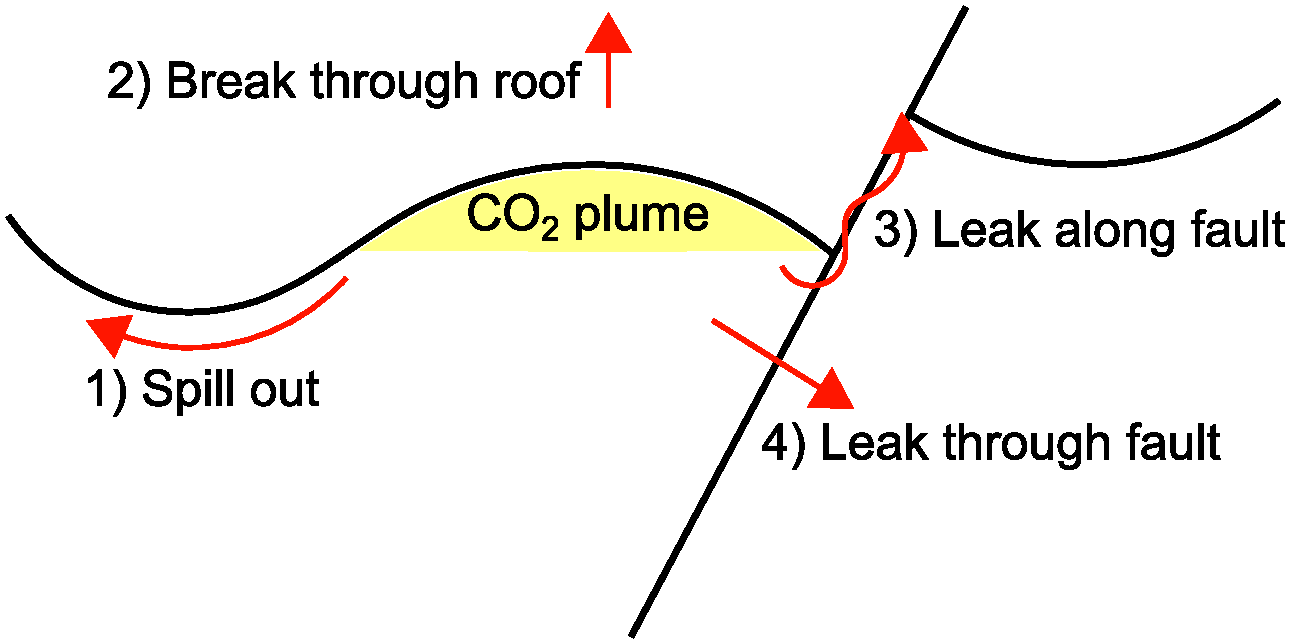
\includegraphics[width=\textwidth]{figures/leakage.pdf}
			\caption{
			Different leakage scenarios for a \ce{CO2} storage project which are subject to uncertainty. To prevent a spill out of the storage formation \textbf{(1)}, the storage capacity must be estimated. A break of \ce{CO2} through the formation's roof \textbf{(2)} depends on seal properties and knowledge of fracture pressures (see figure \ref{fig:compaction}). Evaluation of leakage along \textbf{(3)} or through \textbf{(4)} a fault requires the analysis of juxtaposition and smearing. Sub-seismic faults represent an additional risk. Still, the highest risk of leakage exists in close proximity to wells (Figure based on lecture notes, lecture by K. Indrevær \& A. Braathen, 15.6.2017).
			} \label{fig:leakage}
		\end{minipage}
	\end{minipage}
\end{figure}
	


\end{myblock}\vfill					
					
					
\begin{myblock}{Outlook \& Motivation}
		\begin{minipage}[t]{0.72\textwidth}
			\vspace{0pt}
			Marco studies \textbf{Georesources Management} in Aachen. During his various stays in Norway -- two semesters in Stavanger and summer courses in Oslo and Longyearbyen -- he became passionate about \textbf{risk} and \textbf{decision analysis}. Currently he is writing his master thesis in the field of\textbf{ geologic modelling and uncertainty quantification} in exploration. His focus will be on the application of a \textbf{value of information (VOI)} approach. A specific project to test assumptions and models would be beneficial. The high potential of future \textbf{\ce{CO2} storage projects} provides a suitable case for application. The mentioned methods are believed to contribute to urgently needed \textbf{cost reduction} and \textbf{risk management} of CCS projects.
		\end{minipage}\hfill
		\begin{minipage}[t]{0.23\textwidth}
			\vspace{0em}
			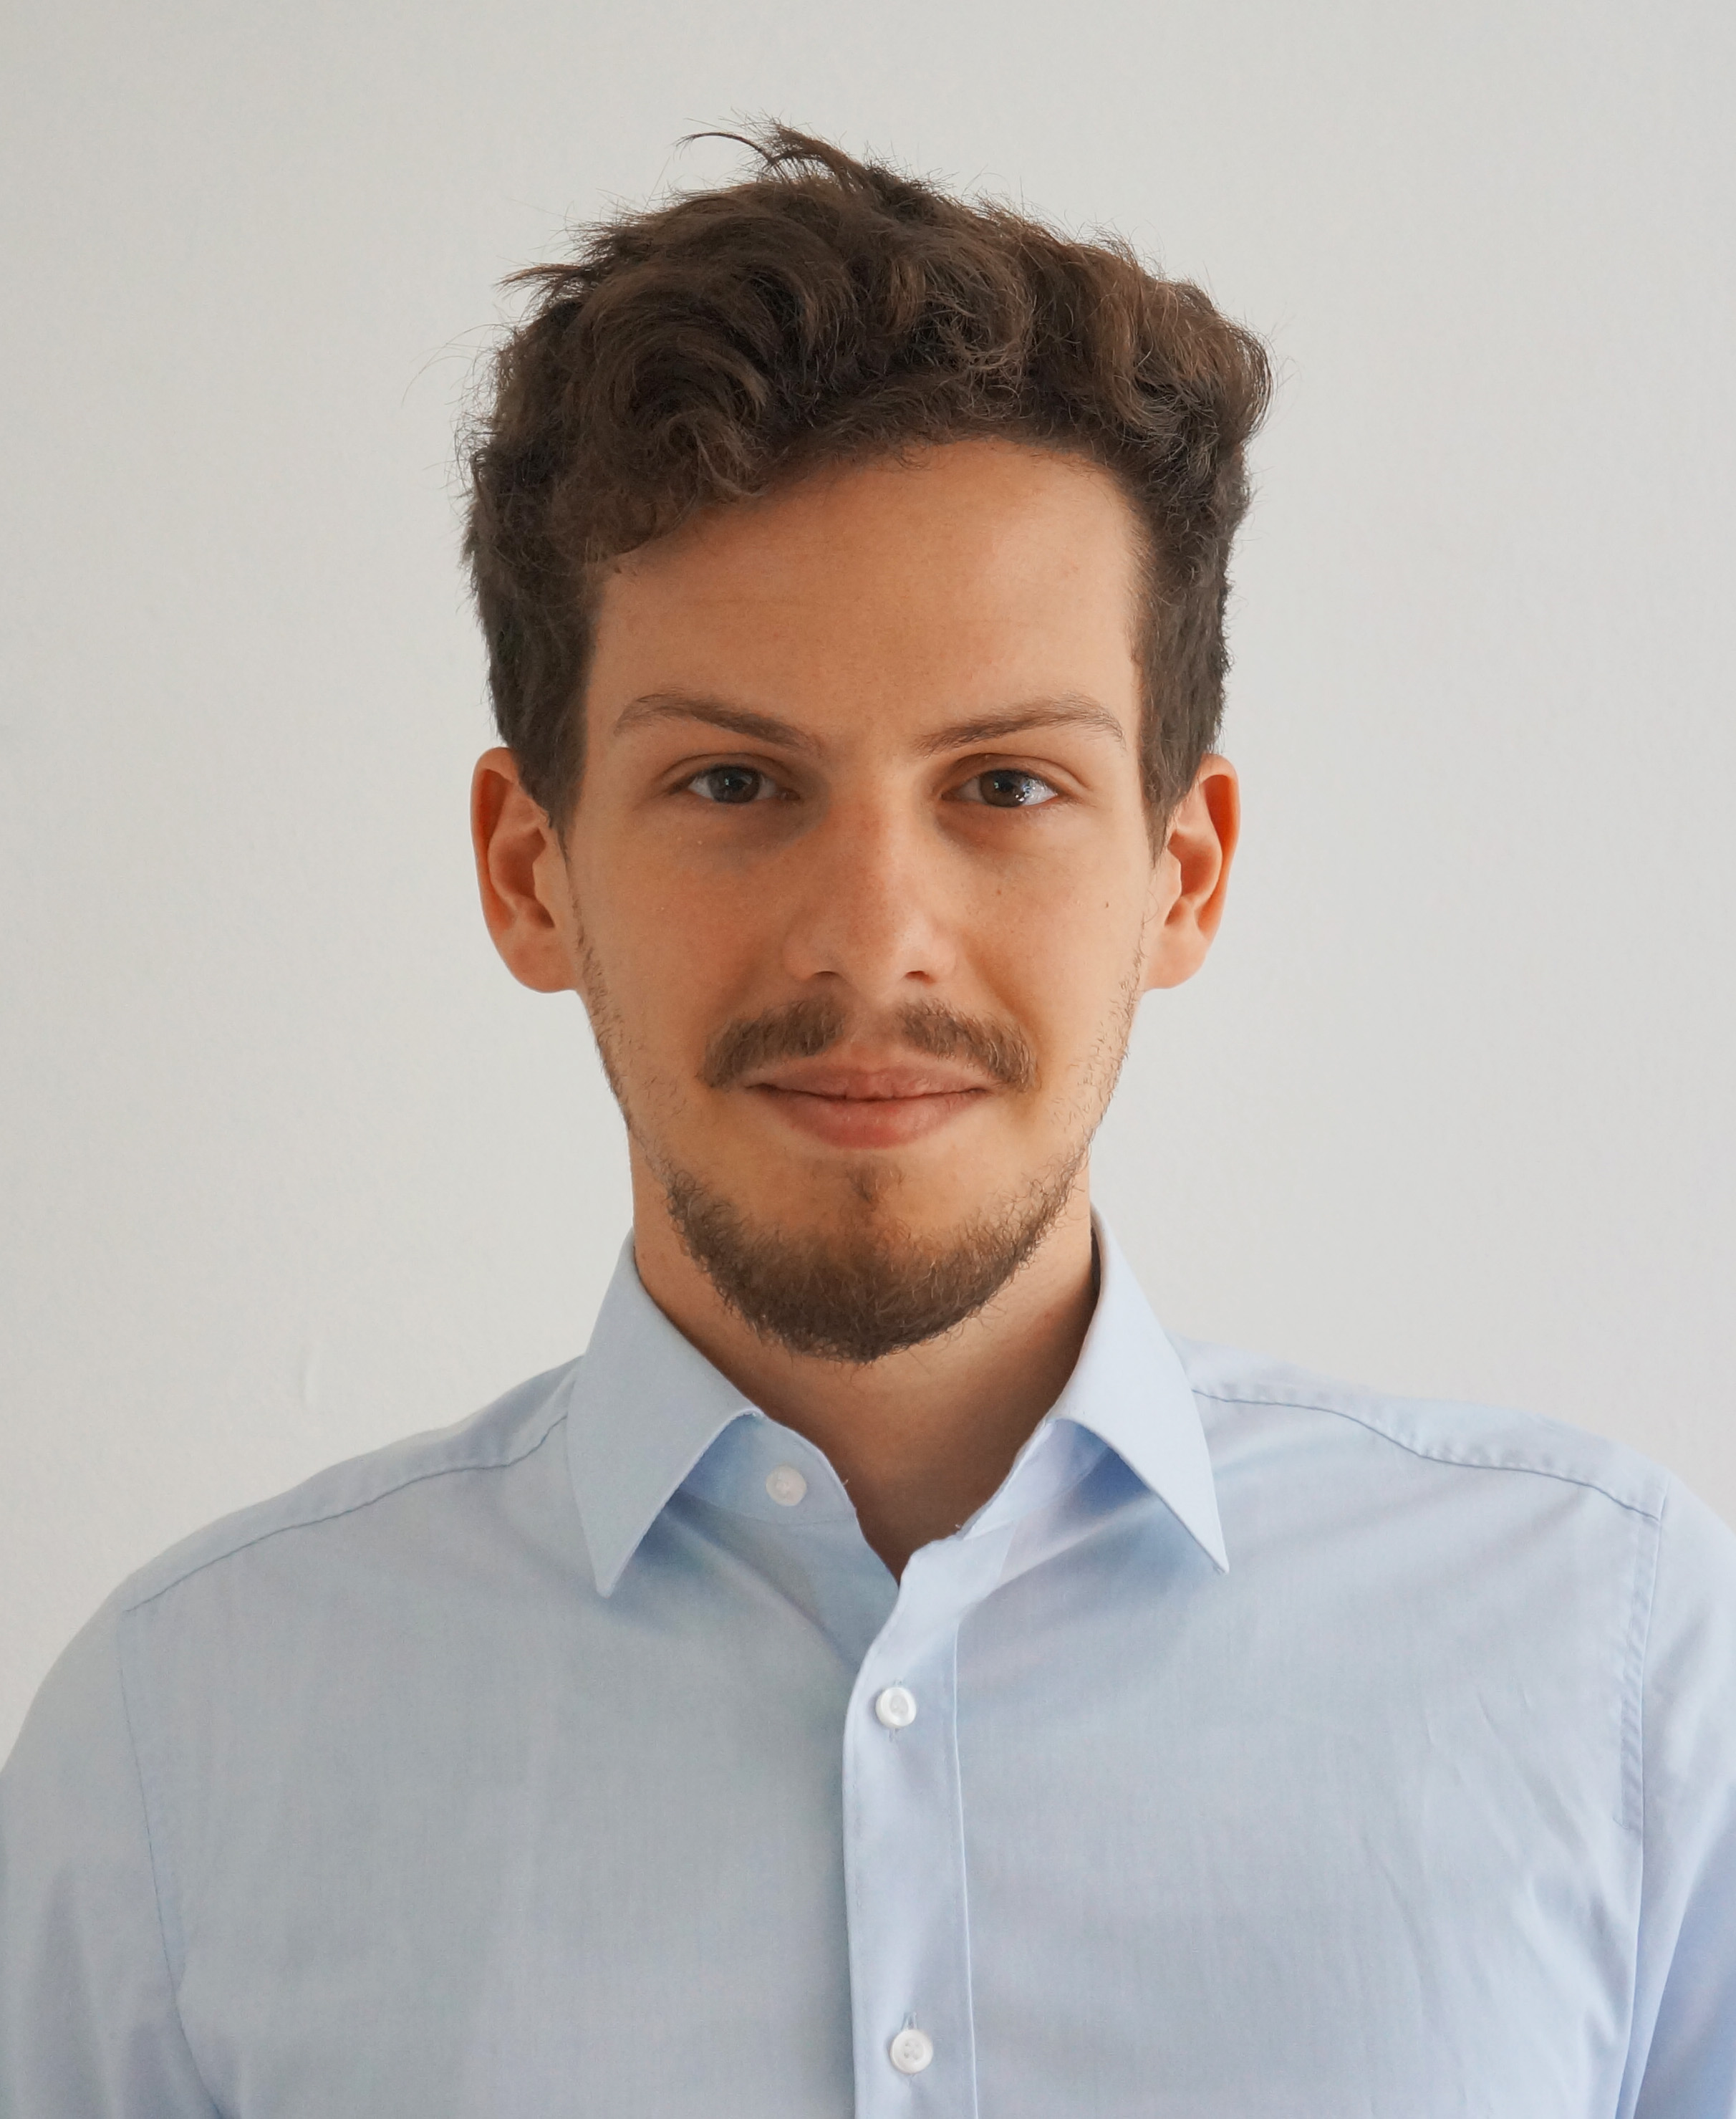
\includegraphics[width=1\textwidth]{figures/author}
			\vspace{0.5em}
		\end{minipage}
		
%			\vspace{0.5em}



\end{myblock}\vfill					
	
					As georesources manager who majored in geoscience I am curious about the structure and dynamics of our earth, but I like to put “these rocks” into a bigger picture. I am not only eager to understand what is going on below our feet, but also to estimate its value to society or economy and to communicate gained knowledge and accompanying risks to decision makers – in order to enable them to make good decisions.

Currently I am writing my master thesis in the field of geologic modelling and uncertainty quantification in exploration. My focus will be on the application of a value of information (VOI) approach and using open source software to demonstrate light weight solutions for high-cost projects.

I am looking for a specific project or data to test the mentioned methods on, preferably in Carbon Capture and Storage (CCS), which I believe has a great potential mitigating the dramatic consequences of climate change.
					
\begin{myblock}{References}
	\footnotesize
	\bibliography{./references}
\end{myblock}


		}\end{minipage}\end{beamercolorbox}
	\end{column}
\end{columns}
\end{frame}
\end{document}
